\chapter{Second Usability Study} \label{chapter:second-iteration}
The previous chapter described how the insights gained during the first study have been translated into redesigned interactions and new interface components. This chapter now looks at how, during the second usability study, the effects of these changes were measured.

\section{Study Design}
% general purpose of study
Whereas the first usability study was mostly about evaluating the high-level aspects of the interface and finding out which areas of the application caused the most serious problems, the second study was more about validating that the introduced changes had a positive impact on the user experience. Furthermore, the general suitability in regards to the envisioned purpose of the system was evaluated. In order to make the results of the first and second study comparable, the setup, especially in regards to the user scenarios, was kept similar.

% prototype - what was tested?
The screens shown in the previous chapter were part of a web-based prototype, that utilized a framework for rapid application development, called AngularJS \cite{_angularjs_????}. Whereas the prototype in the previous study still lacked a couple of important features, such as error messages, the system that was tested in this study was already functional to a large degree. This meant that users could freely interact with the system and therefore the sessions provided a fairly realistic picture of how the system would be used in a real-world environment later on.

% benchmark (metrics and questionnaire)
Additionally to verifying that the introduced changes had indeed improved the usability, a benchmark was established for the very first time. The benchmark was based on the metrics and the post-study questionnaire. Whereas the metrics answered the question whether a goal is reachable within a certain time-frame and by only committing a small number of errors, the questionnaire provided insights into how well the system was perceived in general and which feature areas still need improvement. The benchmark serves as a baseline for other researchers who want to draw on the ideas presented in this thesis and can also be used to evaluate future developments of the system at Babbel.

\subsection{Participants}
The participants of the second usability study were different from the ones during the first study. This was done to ensure that no learning effect would influence the results. Furthermore, it was important that users encountered the concept of version control for the first time when performing the tasks. All participants were selected randomly on a first come first serve basis. As can be seen in Table \ref{table:participants-study2} they represented a diverse group of people. Most of them were part of different language teams and also had different responsibilities within the content creation process. Most participants were content editors and one was a project manager.

As compared to the first study the number of participants was doubled. This was done in order to get more reliable results for the metrics and the newly introduced post-study questionnaire.

\begin{table}[h!]
\centering
\begin{tabular}{|l|l|l|l|}
\hline
\rowcolor[HTML]{EFEFEF}
{\bf Participant} & {\bf Language Team} & {\bf Job Position} \\ \hline
1 & French & Content Editor, QA \\ \hline
2 & Swedish & Content Editor \\ \hline
3 & German, Polish & Project Manager \\ \hline
4 & French & Content \& Image Editor \\ \hline
5 & Portuguese & Content Editor \\ \hline
6 & French & Project Manager \\ \hline
7 & English & Content Editor \\ \hline
8 & Russian & Content Editor \\ \hline
9 & Russian & Content Editor \\ \hline
10 & German & Content Editor \\ \hline
\end{tabular}
\caption{List of Participants}
\label{table:participants-study2}
\end{table}


\subsection{Metrics}
The same quantitative metrics as during the first study were collected. Comparing those might provide helpful insights into what has improved or not.

\begin{itemize}
 \item{\emph{Successful Task Completion}: percentage of tasks that were completed successfully}
 \item{\emph{Time On Task}: time that was needed to perform a task}
 \item{\emph{Error Rate}: participant deviated from “ideal” path of navigation, such as opening the wrong menu.}
 \item{\emph{Scenario Specific Metrics}: such as how long it takes to find the missing translation in Scenario 3 or how quick users discover the create copy function}
\end{itemize}

\subsection{Scenarios}
Scenarios 1 to 3 were identical to the ones used in the first study (as described in Section \ref{sec:scenario-descriptions}). The fourth task has been added to the study in order to lay more focus on the new content representation (main editing view).

The procedure, especially in regards to the scenarios, was kept more or less consistent in order to make comparing the results of the two studies simpler. The interface could be regarded as the independent variable. This means that new results are not influenced by a changed session procedure, but instead can be mostly attributed to the changes in the interface. Of course, given the small number of participants, the different abilities and professional backgrounds of the participants can affect the results as well.

\subsubsection{Scenario 4: Create Exercise and Fill With Content} Add a new memory exercise to this lesson (Link provided). Please don’t edit live content. The title of the exercise should be “awesome memory”. The translation visibility “partial”. Add 3 items to the exercise. Assign random images to the items. Assign all items the speaker role F1. Add all items to the review manager. Finally save your changes.

\subsection{Post-Study Questionnaire}
As an additional means of gathering feedback users were asked to answer a post-study questionnaire. For this, a standardized questionnaire called PSSUQ (Post-study System Usability Questionnaire) was used. PSSUQ was specifically developed for scenario-based usability evaluations at IBM and produces four different scores (one overall score and three sub-scales), which signify how well the computer system was perceived by users \cite{lewis_psychometric_2002}. The goal of utilizing this questionnaire was to reveal potential weak spots of the system, not discovered through the observations, and to get an overall picture of how well the system was perceived. Note that the third version of the questionnaire was used, which consists of 16 items rather than 19 (3 items that contributed rather little to the reliability were removed for this version) \cite{sauro_quantifying_2012}. Each item has to be rated on a scale from 1 to 7, where 1 signifies strong agreement and 7 strong disagreement. Users could also choose to skip an answer. Ultimately, the questionnaire resulted in four scores describing the overall satisfaction with the system as well as the system quality, information quality and interface quality \cite{sauro_quantifying_2012}.

\subsection{Sessions}
Each session was scheduled for one hour. In the beginning participants were introduced to the procedure and the purpose of the study. Afterwards they had to fill in a short questionnaire which asked about their experience with version control systems and the current content authoring tool.

The largest part, going through the scenarios and performing the described tasks, was scheduled to take about 30 minutes. Some users took longer than that, but most finished within the expected time-frame.

Lastly, an open discussion was initiated were questions that arose during the scenarios could be answered and users could provide some general feedback. Usually they were asked about their general impression of the interface and what they liked and disliked most about it. The session concluded with the aforementioned PSSUQ.

\section{Findings}
The following section describes the most important findings of the second usability study. Where meaningful the findings are compared to those of the first study. These include quantitative metrics as well as the discovered usability problems.

\subsection{Metrics}
As during the first study quantitative metrics were recorded. Task completion rate, time on tasks and error rate. Furthermore, a few task-specific metrics were measured. For example for Task 1 it was measured how much time users needed to find the create copy/branch feature. This allowed for a more meaningful comparison as is described in the section below. For task 3 the time for finding the missing translation was recorded.

The tables below show a comparison between the metrics recorded during the first user study and the second. It should be noted that the studies carried out are focused on qualitative findings, which are mostly based on observations and discussions. The metrics only extend and support these findings, but they do not stand for themselves. Because of the relative small sample sizes and partially large variances this data should not be overrated.

\subsubsection{Task Completion Rate}
The task completion rates did not change that much except for Task 1 for which it increased 11 percentage points. One possible explanation is the newly designed warning message, that now offers a direct solution instead of just informing users, which is explained in more detail in Section \ref{sec:live-content-warning}. Unfortunately, 61\% is still an unsatisfactory completion rate. Exactly why it is still so low is hard to tell. Users still seemed to have problems with the dual purpose of merge requests, which serve as a means of reviewing changes. Some users simply forgot to add a reviewer to their requests, others said they would probably send a link to their colleagues and ask them to have a look at the changes.

Another reason for the low completion rate, especially in comparison with the other tasks, might be that users had to get used to the interface at first. The task order was not randomized but always remained the same. A randomized task order might have resulted in a more balanced rate, in particular between Task 1 and 3, which according to the participants were the most difficult tasks.

\begin{table}[h!]
\centering
\begin{tabular}{|l|l|l|l|}
\hline
\rowcolor[HTML]{EFEFEF}
{\bf Scenarios} & {\bf First Study} & {\bf Second Study} & {\bf Difference in pp} \\ \hline
Scenario 1 & 50\% & 61\% & +11 pp \\ \hline
Scenario 2 & 100\% & 94\% & -6 pp \\ \hline
Scenario 3 & 70\% & 72\% & +2 pp \\ \hline
Scenario 4 &  & 100\% &  \\ \hline
\end{tabular}
\caption{Comparison of task completion rates during first and second user study}
\label{table:task-compl}
\end{table}

\subsubsection{Time on Tasks}
As Table \ref{table:time-tasks} shows the biggest difference is again observed for Scenario 1. Participants during the second study needed about 75 seconds less for finishing this scenario than participants in study 1. For Scenario 3, participants needed about half a minute less than during the previous study. Because of the small sample sizes these numbers are not statistically significant and should therefore be taken with a grain of salt.

\begin{table}[h!]
\centering
\resizebox{\textwidth}{!}{%
\begin{tabular}{|l|l|l|l|}
\hline
\rowcolor[HTML]{EFEFEF}
{\bf Scenarios} & {\bf First Study (mean)} & {\bf Second Study (mean)} & {\bf Difference} \\ \hline
Scenario 1 & 367 & 292.25 & -74.75 \\ \hline
Scenario 2 & 128 & 146.57 & 18.57 \\ \hline
Scenario 3 & 395.5 & 369.42 & -26.08 \\ \hline
Scenario 4 &  & 280 &  \\ \hline
\end{tabular}
}
\caption{Time on tasks (in seconds)}
\label{table:time-tasks}
\end{table}

\subsubsection{Errors}
Even though the other metrics show most improvements for Task 1, this is not the case for the error rate. Here, there is only a slight decrease of errors for Task 1, whereas errors during the other tasks (2 and 3) have halved. A possible explanation for this might be the changed terminology, which allowed users to better orient themselves (action verbs and more everyday language than technical terms). It seems there was less trial and error when finding the right feature. The observations support this assumption, e.g. there were fewer users asking things like “What is a pull request?”. Nevertheless, users still encountered serious usability issues that led to confusion and errors. Those are described in more detail below (Section \ref{sec:discovered-usability-issues}).

\begin{table}[h!]
\centering
\begin{tabular}{|l|l|l|l|}
\hline
\rowcolor[HTML]{EFEFEF}
{\bf Scenarios} & {\bf Study 1} & {\bf Study 2} & {\bf Difference in Errors} \\ \hline
Scenario 1 & 2.2 & 1.87 & -0.33 \\ \hline
Scenario 2 & 1.6 & 0.5 & -1.1 \\ \hline
Scenario 3 & 4.2 & 2.12 & -2.08 \\ \hline
Scenario 4 &  & 0.5 &  \\ \hline
\end{tabular}
\caption{Comparison of error rates during first and second user study }
\label{table:second-study-error-rate}
\end{table}

\subsection{Impact of Design Changes}
The major changes implemented for this study had different levels of impact. Some of the changes were quite noticeable during the sessions whereas others are harder to validate.

\subsubsection{Navigation Bar \& Changed Terminology}
The new navigation bar did not attract a lot of attention, which is probably a positive sign. The reduced error rate could at least be partially attributed to the improved naming and the icons (Table \ref{table:second-study-error-rate}). In general, there seemed to be less trial and error when users navigated the application. During the previous study remarks like "What is a pull request?" and "I'm just going to click through, I have no idea" suggested that there is a usability problem. This time, these remarks were much less frequent. Especially the new terms "working copy" and "merge request" seemed to be much better understood than their predecessors. Furthermore, using action verbs to highlight what a feature can do instead of passively describing it cleared things up as well.

% \subsubsection{Visualisations}
% The new visualisations did not result in a noticeable change. Since the new terminology was more straightforward the need for visualisations could have been reduced by that as well (Figure \ref{fig:approve-request}).

% \begin{figure}[h!]
%  \centering
%  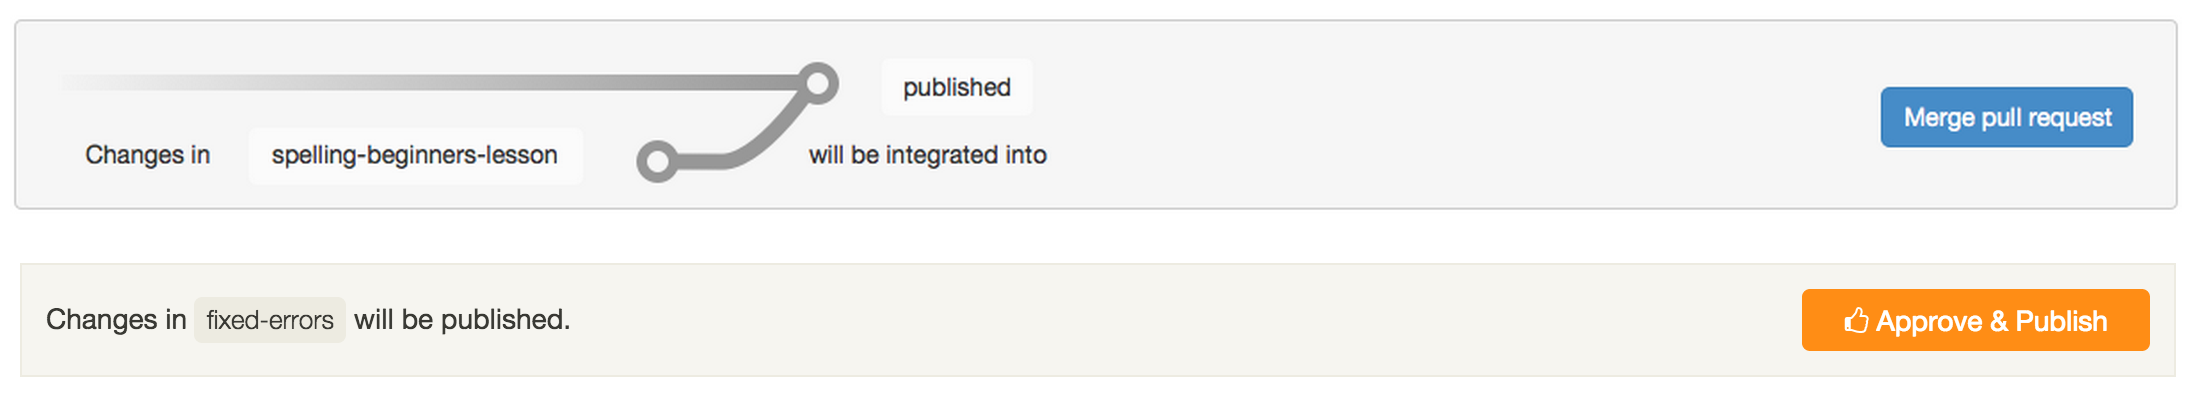
\includegraphics[width=\textwidth]{second-iteration/changes/approve-request}
%  \caption{Approving a request old vs. new}
%  \label{fig:approve-request}
% \end{figure}

\subsubsection{Saving Process}
A positive outcome of the newly added saving shortcut was that it was used a lot. The downside on the other hand was that some users got confused by the existence of two different saving features. The shortcut save sped up editing and users did not seem to miss the list of changes they would got with the "advanced" saving feature. What has become apparent is that the old saving feature, which concept-wise, is very much inspired by the staging area of version control systems, might not be the most intuitive solution for content editors. In programming there is often a need of touching many files at once to implement a new feature. In content editing this is seldom the case. Changes are usually logically tied to a single lesson.

\subsubsection{Live Content Warning} \label{sec:live-content-warning}
Task 1 asked users to apply two small changes inside a lesson. The difficulty was that they were not supposed to edit the live content. That meant that they had to create a copy (branch) of the content first, make the changes, save them and finally merge the copy with the public content again. During the first study participants wasted a lot of time finding the create branch/copy feature after they had been alerted to not edit the live content. As Figure \ref{fig:avg-time-task1} shows this time could be greatly reduced through the new design in the second study. The dark grey bars show the moment in time when users discovered the feature. During the first study users spent almost half of the time with finding this feature whereas during the second study they discovered it a lot earlier. This also had an effect on the average time taken for Task 1 in total and the completion rate. These improvements are probably due to the redesign of the warning message as described in the previous chapter (Figure \ref{fig:live-data-warning}).

\begin{figure}[h!]
 \centering
 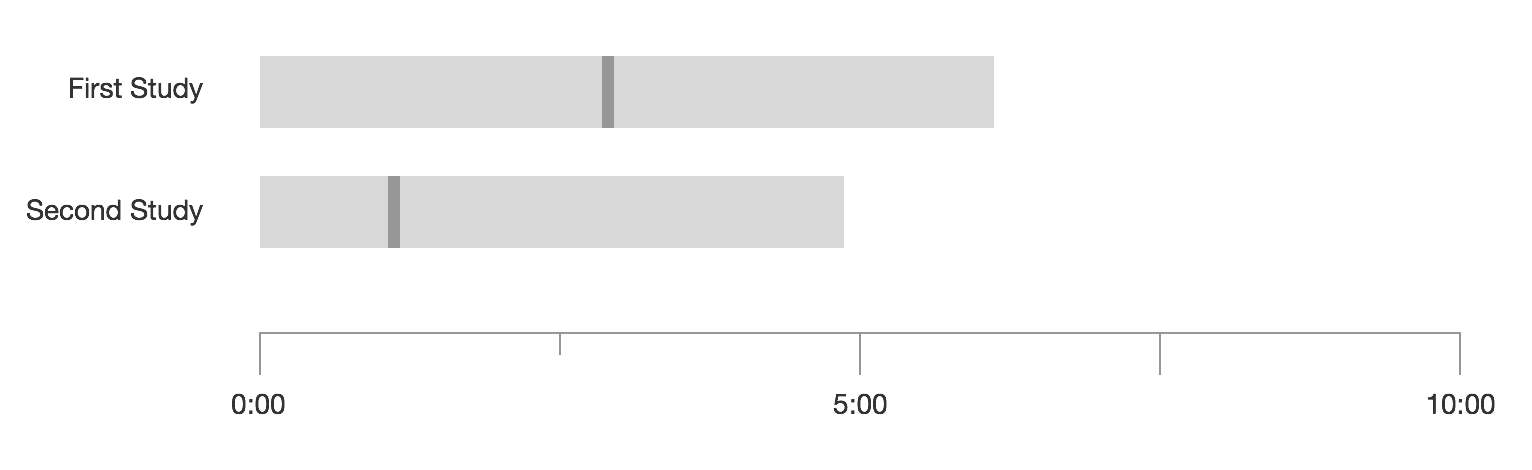
\includegraphics[width=12cm]{second-iteration/plot-branch-creation}
 \caption{Average task completion time and time of branch/copy creation}
 \label{fig:avg-time-task1}
\end{figure}

\subsubsection{Content Representation}
In general the new content representation performed quite well. This became apparent in Task 3 when users had to find a missing translation. Whereas, during the previous study, some users had problems locating this missing field within the content representation (because it was initially hidden), this was no longer a problem with the new design. Once users had arrived at the content of a lesson and selected the right language they could locate the missing translation quite quickly. The only noteworthy issues of the new design were malfunctioning popovers (did not close automatically) and labels that looked placeholders and were therefore selected by some users (instead of the actual input field).

%figure here of old new content representation (finding translation)


%\subsection{Scenario 2}
%Scenario 2, as during the first round of user tests, seemed to be the easiest one. 94\% completed the task with only 0.5 errors on average. This shows that the two main views needed for solving this task have a low number of usability issues. The reduced number of errors could also be attributed to the new naming. Instead of “Pull Requests” the feature was called “Review Requests” and instead of “Merge Pull Request” the command for merging changes was now called “Approve \& Publish” (Figure \ref{fig:approve-request}).

%\subsection{Scenario 3}
%Scenario 3 seemed again to be the most tricky one. Users especially struggled with finding the missing translation. Even though the new content representation made it easier to find the missing translation once they had navigated to the right lesson, most of them still got stuck in the list of changes and tried finding the missing translation there. Only 2 out of 10 users noticed that a translation that was forgotten could not show up in a list of changes, because it was never altered. The quotes below illustrate how users felt during this scenario.

%\subsection{Scenario 4}
%The observations of scenario 4 cannot be compared to the first study since it was introduced only for this study. The purpose was to assess the usability of the changed content representation and the ease of adding new content. This task, as task 2, posed relatively few problems to users. The only noteworthy issues are that popovers did not close automatically when clicked outside and labels that were confused with placeholders and therefore selected by some users (instead of the actual input field).


\subsection{Discovered Usability Issues} \label{sec:discovered-usability-issues}
Even though several usability issues were fixed as compared to the first study, there were also a lot of new ones coming up. Some of this might be due to the fact that users could now freely interact with the tool and were not constrained by the prototype design as in the first study. In total, the number of rather severe issues (Severity score of 10 or 5)  was reduced from 15 in the previous study to 11 during the second study. Also the impact of most issues was lower this time, which can be attributed to less users experiencing the problem.

The following section lists the usability issues discovered during the test sessions. As for the first study, the impact score by Sauro and Lewis \cite{sauro_quantifying_2012} was calculated for each issue and the tables are sorted by the highest impact scores. Please note, in order to avoid confusion later on, the issue numbers are continuous and thus start with 27.

% this is now described in the first study
% The following section describes the usability problems that have been discovered by observing participants performing the different scenarios. They are grouped by feature areas of the application and the most important issues are shortly explained. In order to rank the issues by their impact on the user experience a severity score was used, as suggested by Sauro and Lewis \cite{sauro_quantifying_2012}. The most severe issues, which prevented users from completing the tasks, were given a score of 10. 5 points were assigned if the issue caused a significant delay or frustration. 3 points were allocated for minor issues and just 1 point for improvements suggested by participants. To create an impact score the severity was multiplied by the frequency of users who experienced the problem (severity * frequency / 10). A frequency of 40\% means that 4 of 10 users encountered the problem, independent of whether they ran into the issue more than once. The scale ranges from 100 (most severe problem, experienced by all users) to 1 (suggestion by a single user).

\subsubsection{Working Copies}
Working copies, which were previously called branches, were in general quite well understood. Nevertheless, they also caused some usability issues. A common misconception was that a working copy only consists of one lesson, where in reality it contains the whole language package (repository).
Furthermore, the interface did not provide appropriate feedback when errors occurred, the feedback was either too general or completely non-existent (Table \ref{table:issues-copies}). Additionally, some users did not realize that after creating a new copy it was already selected. The name in the dropdown changed, but it is barely noticeable if you do not know where to look.

% \begin{displayquote}
% "I like that I get all this information." \textit{Participant 8}
% \end{displayquote}

\begin{table}[h!]
\centering
\begin{tabular}{|r|p{7cm}|r|r|r|}
\hline
\rowcolor[HTML]{EFEFEF}
{\bf \#} & {\bf Usability issue} & {\bf Severity} & {\bf Frequency} & {\bf Impact} \\ \hline
27 & User does not know whether newly created copy is already selected & 10 & 40\% & 40 \\ \hline
28 & No error message when copy with existing name is created & 10 & 20\% & 20 \\ \hline
29 & Error message too general when spaces are used in copy name & 5 & 30\% & 15 \\ \hline
30 & Users have wrong understanding of working copy (think that lesson is copied) & 3 & 40\% & 12 \\ \hline
31 & Copies accumulate quickly - results in long dropdown list which is hard to scan quickly & 1 & 20\% & 2 \\ \hline
\end{tabular}
\caption{Usability issues related to working copies}
\label{table:issues-copies}
\end{table}

\subsubsection{Merge Requests}
As Table \ref{table:issues-merge} shows merge requests were the root of various usability issues. First of all, there was a missing error message when users tried to create a merge request based on a copy that did not contain changes (as compared to the \textit{published} content). This happened when users forgot to save and went straight to the merge request view. Furthermore, the reviewer functionality was not always discovered, because it is not prominent enough.

\begin{table}[h!]
\centering
\begin{tabular}{|r|p{7cm}|r|r|r|}
\hline
\rowcolor[HTML]{EFEFEF}
{\bf \#} & {\bf Usability issue} & {\bf Severity} & {\bf Frequency} & {\bf Impact} \\ \hline
32 & User tried creating merge request before saving (no error message) & 10 & 20\% & 20 \\ \hline
33 & User does not know how to let colleague review changes & 10 & 10\% & 10 \\ \hline
34 & When approving a merge request and commenting first comment confirmation is forgotten & 3 & 30\% & 9 \\ \hline
35 & Commenting in request detail view (diff) does not result in feedback & 3 & 10\% & 3 \\ \hline
36 & The list of requests does not show the reviewers at a glance & 3 & 10\% & 3 \\ \hline
\end{tabular}
\caption{Usability issues related to merge requests}
\label{table:issues-merge}
\end{table}

\subsubsection{Diff}
The diff view, which was only subject to a small set of changes as compared to the last iteration, caused the most problems. This is surprising, since these issues have not been discovered during the first study. Maybe this time users were better able to articulate themselves or the root of their frustration was more obvious in a fully functioning system. The main problem with the diff view, which design is heavily inspired by Github, was that it does not provide enough context. The listed changes were only of limited value, if not meaningless, without the context they originated from (lesson or exercise). In programming a single method or class can usually be assessed in isolation, but for language learning it is much more important to know the context of a certain element.

% \begin{displayquote}
% "I’m totally lost inside this view." \textit{Participant 3}
% \end{displayquote}


\begin{table}[h!]
\centering
\begin{tabular}{|r|p{7cm}|l|l|l|}
\hline
\rowcolor[HTML]{EFEFEF}
{\bf \#} & {\bf Usability issue} & {\bf Severity} & {\bf Frequency} & {\bf Impact} \\ \hline
37 & It is hard to deduce the structure of the content from the diff view & 10 & 90\% & 90 \\ \hline
38 & Diff view is missing context (i.e. text that was translated) & 5 & 80\% & 40 \\ \hline
39 & It is not clear how to get from the diff view to the content & 10 & 20\% & 20 \\ \hline
40 & Change description is above red box in diff view which is confusing (what has changed?) & 5 & 30\% & 15 \\ \hline
\end{tabular}
\caption{Usability issues related to the diff view}
\label{table:issues-diff-2nd}
\end{table}


\subsubsection{Saving process}
The saving process, as described before, now offered two options, a direct save below the editing view and a more advanced option where users would see their changes again. The positive aspect is that many users used the new saving feature and most of them did not even notice that there were two options. The flipside of this is, when users did notice there were two options, they were severely confused.
Two more things that caused problems were again related to feedback and error messages (Problem 1 \& 2, Table \ref{table:issues-saving}. When users try to save without entering a description (commit message) the input field turns red, but there is no explanation on why this is needed. Furthermore, after saving changes using the advanced option, the \textit{blank slate} \cite{_blank_????} appears telling users "no unsaved changes". This is rather confusing, because the blank slate is a design pattern that is aimed at helping users out in case they encounter a dead-end or empty view. Instead there should be a confirmation informing users about a successful save.

\begin{table}[h!]
\centering
\begin{tabular}{|r|p{7cm}|l|l|l|}
\hline
\rowcolor[HTML]{EFEFEF}
{\bf \#} & {\bf Usability issue} & {\bf Severity} & {\bf Frequency} & {\bf Impact} \\ \hline
41 & Difference between two saving features unclear & 10 & 30\% & 30 \\ \hline
42 & User tried saving without entering description & 3 & 90\% & 27 \\ \hline
43 & No unsaved changes? Blankslate after save is confusing - no confirmation (same for shortcut) & 5 & 50\% & 25 \\ \hline
44 & There should be a suggestion after saving changes what to do next & 1 & 30\% & 3 \\ \hline
\end{tabular}
\caption{Usability issues related to the saving process}
\label{table:issues-saving}
\end{table}

\subsubsection{Main Editing View}
As mentioned before there were relatively few problems arising in the main editing view. The most severe one only influenced a single user who got confused because the translation column was showing a different language than the one she had selected before. The view does not "remember" the display language setting. It always switches back to a default when the user comes back from a different view. The other issues were only minor ones that users could easily recover from. Nevertheless they should be fixed to improve the editing workflow.

% \begin{displayquote}
% "The interface is clear and friendly." \textit{Participant 6}
% \end{displayquote}

\begin{table}[h!]
\centering
\begin{tabular}{|r|p{7cm}|r|r|r|}
\hline
\rowcolor[HTML]{EFEFEF}
{\bf \#} & {\bf Usability issue} & {\bf Severity} & {\bf Frequency} & {\bf Impact} \\ \hline
45 & Clicked on label that looked like placeholder in order to enter data & 3 & 40\% & 12 \\ \hline
46 & There is only one (not obvious) way of closing a popover & 3 & 30\% & 9 \\ \hline
47 & A comment functionality was suggested & 1 & 10\% & 1 \\ \hline
\end{tabular}
\caption{Usability issues related to main editing view}
\label{table:issues-main-editing-view}
\end{table}

% miscellaneous?

%\section{Positive Aspects}
%Despite the long list of usability issues there were also several positive aspects observed during the sessions. In general users seemed to be less confused with the whole version control workflow (creating copies, editing, merging). The warning messages and information provided in the interface helped users to get back on the right track in case they got lost. This, for example, was specifically expressed by Participant 9 when she encountered the live content warning ("I like that I get all the information here"). Furthermore,  changes such as the new content representation and the new saving feature had a positive impact.

\subsection{Post-study Questionnaire}
Table \ref{table:post-study-scores} shows the resulting  scores of the Post-Study System Usability Questionnaire (PSSUQ). The lower the value, the more satisfied users were with the particular aspect of the system. These scores are based on the mean of 16 items that comprise the PSSUQ. The list below shows which items contribute to which score. The complete catalog of questions together with the average ratings can be found in the appendix (Table \ref{table:post-study-scores}).

\begin{itemize}
 \item \textit{Overall:} Average of items 1 through 16
 \item \textit{System Quality:} Average of items 1 through 6
 \item \textit{Information Quality:} Average of items 7 through 12
 \item \textit{Interface Quality:} Average of items 13 through 15
\end{itemize}

As can be seen the overall feedback was quite positive although there is still room for improvement (2.83 vs. the neutral value 4). Participants seemed to be especially pleased with the interface quality, which basically describes the aesthetic and functional quality of the system. The high score could partially be due to the sharp contrast between the existing content authoring tool, which is very cluttered, and the new one. System quality, which assesses ease of learning and the general usability received a good average score as well (2.51). The fourth score, information quality, did not fare as well as the other ones (3.38). Information quality describes how much documentation is offered, how well error messages are designed and how easy it is for users to recover from their mistakes. The reasons for the low score are probably a non-existent documentation and still a lot of missing error messages, as described earlier. Some users ran into issues where the system did not react to their input but also did not provide any feedback which would have allowed users to recover.

\begin{table}[h!]
\centering
\begin{tabular}{|l|l|}
\hline
\rowcolor[HTML]{EFEFEF}
{\bf 4 scores} & {\bf Rating (mean)} \\ \hline
Overall & 2.7 \\ \hline
System Quality & 2.51 \\ \hline
Information Quality & 3.31 \\ \hline
Interface Quality & 2.07 \\ \hline
\end{tabular}
\caption{Average scores for the 4 dimensions}
\label{table:post-study-scores}
\end{table}

\subsection{Conclusion}
What has become apparent by looking at the findings above is that almost all changes that were introduced had a positive impact. For some of these improvements the metrics speak for themselves: the reduced time for Task 1 due to the redesigned live content warning and the lower error rate (all tasks) due to an improved navigation bar and a better terminology. For changes like the new saving feature and the improved content representation a shift in behaviour could be observed. But, these changes also introduced new problems. Even though the saving shortcut was used a lot and users did not have to search for a save button anymore as in the previous study, those that noticed the presence of two disparate saving mechanisms were usually confused by it.

Most surprising was the fact that severe usability issues were discovered related to the diff view, which did not surface during the last study, even though the design had only changed in a few details. The fact that other problems had been eliminated, for example with the content representation, might have contributed to making these problems more obvious.

In general it is to say that testing a more ore less functioning application is very different from testing a prototype. Users are much more demanding and expect the interface to work properly. On the other hand it needs less interference by the moderator and therefore more problems are discovered. Users can freely move inside the application and might do things that the designers of the system did not conceive before. From this, interesting new ideas can evolve.

The next chapter presents the final design of the system, which is based on the findings of this usability study.


% \section{Next Steps}
% As might have become clear in the previous sections there is still a lot to improve. Particularly the diff view and the saving process still have some serious problems. Furthermore, there are a lot of smaller usability issues that need to be fixed. The next chapter presents the final design of the authoring system, which is based on the findings of this usability study.

%\section{Recommendations \& Next Steps}
%- unite saving features (with old/new state in table view)
%- redesign diff view
%Maybe in final conclusion?
%- thesis ands here
%- now it is for others to pick up and continue the work. the project has shown that version control can be a valuable extension of authoring systems. it is a powerful mechanism that can make life simpler for many users dealing with large amounts of content or data that is also changing constantly. It is ripe for taking the step outside the programming world.

%Despite a lot of usability issues being discovered during the last study, in overall the user satisfaction was quite high (2.7 overall rating, 2.07 interface quality).


%"interface is clear and friendly" "this is so much better than github" "you get an excellent overview"

% - two main areas of improvement: diff and saving
